% Verbatim from minor_report/chapters/chapter_4_results.tex lines 917-1038 (retired report),
% headings demoted by 1 level(s). Do not edit here; edit the source of the numbers.

YOLO was evaluated independently of either SLAM integration on all four dynamic
no-floor-texture rosbags. Ground-truth object poses came from
\repo{/world/default/pose/info}; because that topic's message headers are zero,
its rosbag receive times were mapped to simulation time by interpolation against
the recorded \repo{/clock} stream. Known model meshes were transformed into the
camera frame and projected into \repo{cam0} to form two-dimensional boxes.
Sampled overlays from every bag were inspected before calculating metrics and
showed spatially plausible agreement between the projected boxes and visible
objects.

\subsubsection{Bounding-Box Detection and Localization}
\label{sec:yolo-bbox}

The evaluation used 9,860 camera frames, confidence threshold 0.35, NMS IoU
threshold 0.50, and matching IoU threshold 0.50. Ground-truth
boxes smaller than 12 pixels on either side were omitted; heavily occluded
ground-truth boxes and predictions explained by explicitly unlabelled scenery
were ignored rather than counted as errors. Table~\ref{tab:yolo-performance}
reports per-dataset results and a micro-average formed by pooling TP, FP, and FN
counts across all frames.

\begin{table}[htbp]
\centering
\caption[Offline YOLO performance against projected Gazebo object ground truth.]{Offline YOLO performance against projected Gazebo object ground truth.
This is a detector-capability measurement, not an evaluation of delivery to the
online SLAM filters.}
\label{tab:yolo-performance}
\resizebox{\textwidth}{!}{%
\begin{tabular}{lrrrrrrrr}
\toprule
Dataset & Frames & TP & FP & FN & Precision & Recall & F1 & Moving recall \\
\midrule
Dynamic 00/000 & 2,347 & 9,987 & 4,826 & 5,900 & 0.674 & 0.629 & 0.651 & 0.617 \\
Dynamic 00/001 & 2,236 & 10,158 & 4,265 & 6,868 & 0.704 & 0.597 & 0.646 & 0.599 \\
Dynamic 01/000 & 2,564 & 8,142 & 4,226 & 6,064 & 0.658 & 0.573 & 0.613 & 0.568 \\
Dynamic 02/000 & 2,713 & 8,661 & 3,743 & 6,502 & 0.698 & 0.571 & 0.628 & 0.581 \\
\midrule
Pooled & 9,860 & 36,948 & 17,060 & 25,334 & 0.684 & 0.593 & 0.635 & 0.591 \\
\bottomrule
\end{tabular}}
\end{table}

The pooled evaluation contains 62,282 scored ground-truth boxes, of which 46,491
are moving, plus 34,476 projected boxes excluded as heavily occluded. The model
produced 58,776 raw predictions. Mean image coverage was 10.42\% for all scored
ground truth, 7.88\% for moving ground truth, and 9.07\% for predictions. At the
stated thresholds, the detector misses approximately 41\% of scored moving
objects; moving-object recall ranges from 0.568 to 0.617 between datasets.
Conversely, the results demonstrate that the trained model can produce detections
on every recorded bag. They do not contradict the zero-box VINS+YOLO logging
anomaly: offline detector capability and online message delivery/timestamp
matching are different mechanisms. Average precision is not reported because
this evaluation retained predictions only above a single confidence threshold.

\begin{figure}[htbp]
  \centering
  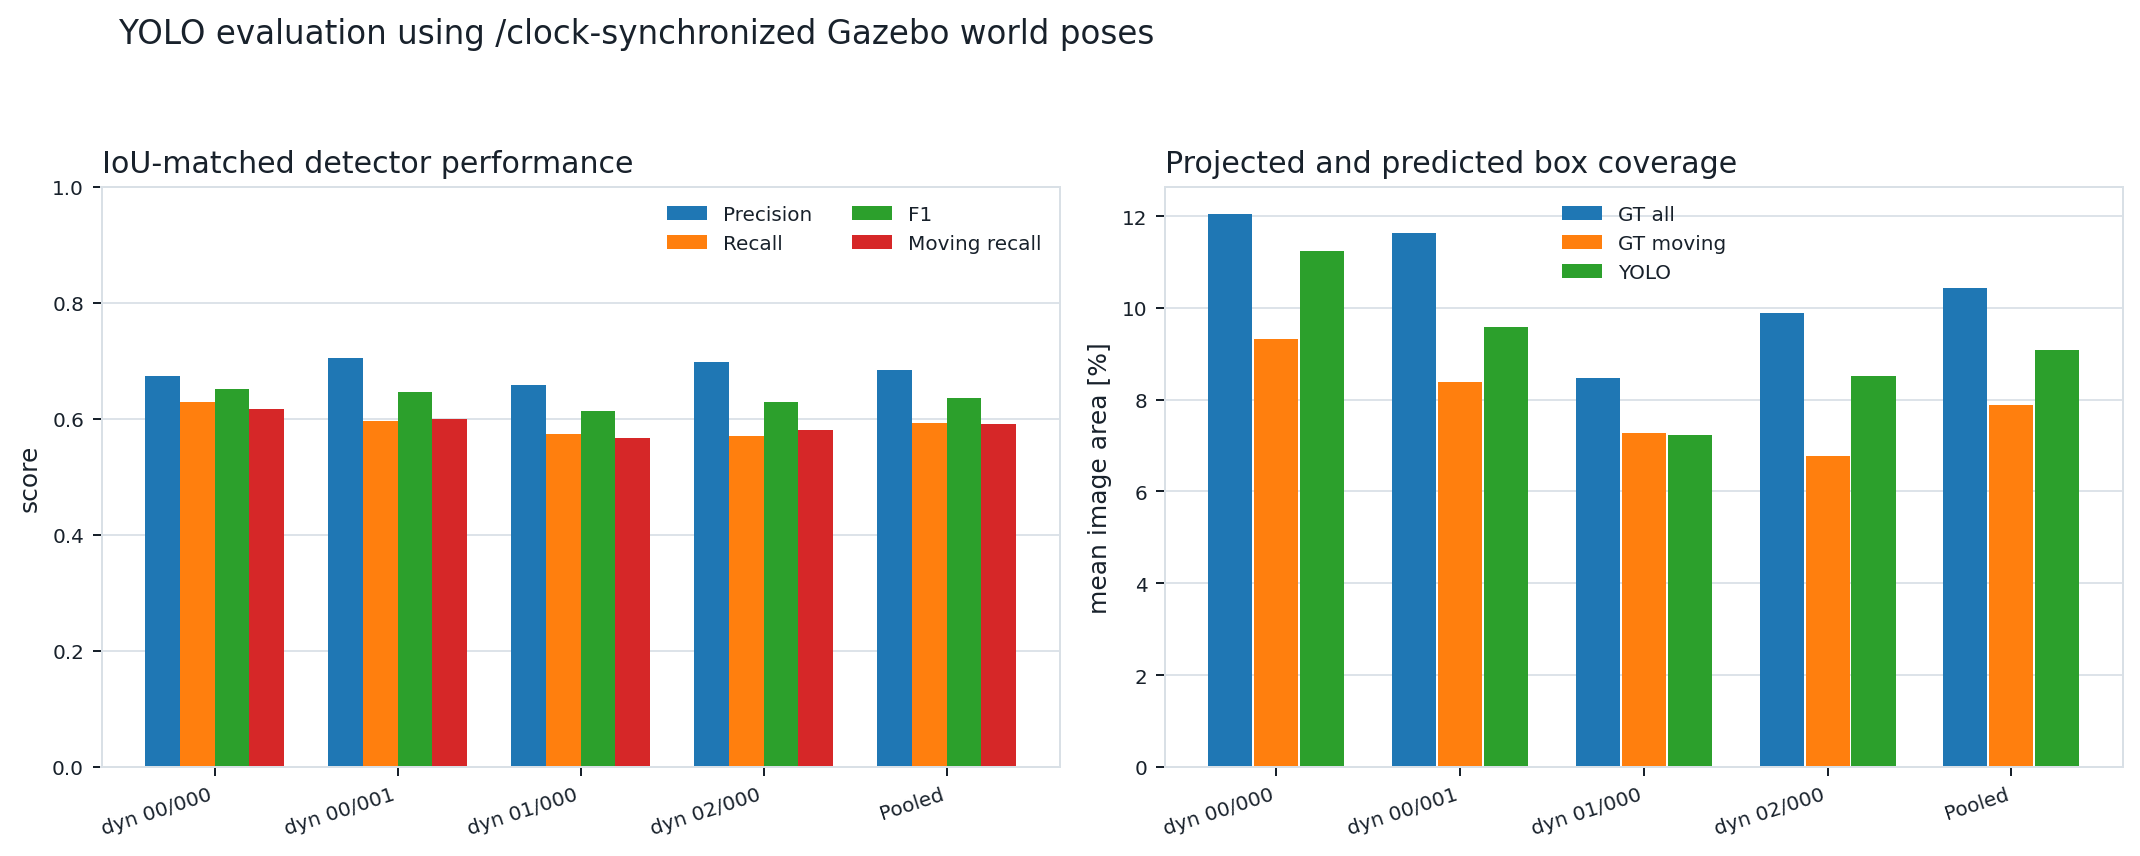
\includegraphics[width=\textwidth]{../../../output/yolo_eval/summary_light.png}
  \caption[Per-dataset and pooled detector scores and box-area coverage.]{Per-dataset and pooled detector scores and box-area coverage. Pooled
  precision, recall, F1, and moving-object recall are calculated from pooled
  counts, rather than by averaging the four displayed dataset scores.}
  \label{fig:yolo-performance-summary}
\end{figure}

\begin{figure}[htbp]
  \centering
  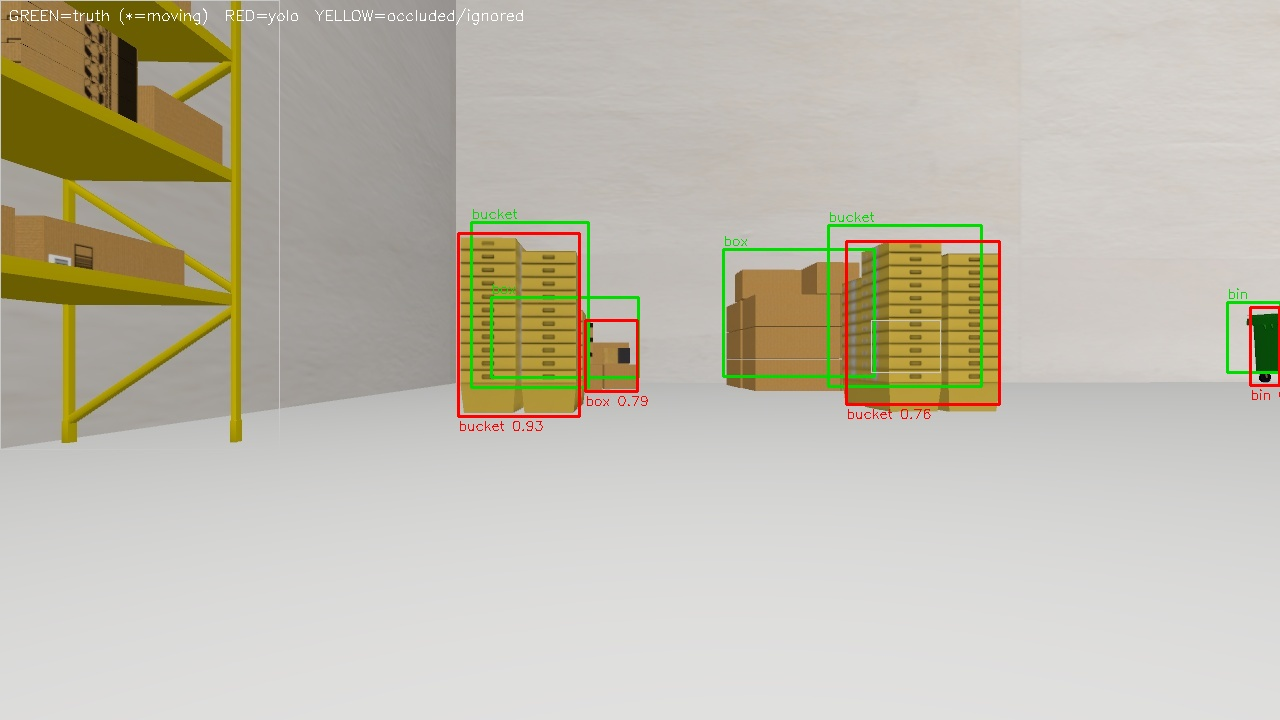
\includegraphics[width=\textwidth]{../../../output/yolo_eval/dyn_00_001/overlay/01116.jpg}
  \caption[Representative validation overlay used before accepting the offline metrics.]{Representative validation overlay used before accepting the offline
  metrics. Green boxes are projected ground truth and red boxes are YOLO
  predictions. A \textbf{yellow} box is a ground-truth object that a nearer
  object covers by more than \SI{70}{\percent}; it is excluded from scoring, so
  the detector is neither credited for finding it nor penalised for missing it.
  Only the green boxes are scored. An asterisk marks a ground-truth object
  classified as moving from its world-pose history.}
  \label{fig:yolo-ground-truth-overlay}
\end{figure}

\clearpage
\subsubsection{Object-Class Assignment Conditional on Localization}
\label{sec:yolo-classification}

This experiment is not whole-image classification: an image can contain many
objects, and the model outputs a class for each predicted bounding box. To keep
class assignment separate from localization, predictions and ground-truth boxes
were greedily associated by IoU $\geq0.50$ without requiring their classes to
agree. Classification was then evaluated only on the 37,061 localized object
pairs. Missed ground-truth objects and unmatched predictions remain bounding-box
detection errors in Section~\ref{sec:yolo-bbox}; they are not treated as an
additional semantic class here.

\begin{table}[htbp]
\centering
\caption{Object-class assignment conditional on successful IoU association,
pooled across the four dynamic datasets.}
\label{tab:yolo-classification}
\begin{tabular}{lrrrr}
\toprule
Class & Associated objects & Precision & Recall & F1 \\
\midrule
Bin & 2,639 & 1.000 & 1.000 & 1.000 \\
Box & 28,076 & 0.996 & 0.999 & 0.998 \\
Bucket & 6,346 & 0.996 & 0.983 & 0.989 \\
\midrule
Macro average & 37,061 & 0.997 & 0.994 & 0.995 \\
\bottomrule
\end{tabular}
\end{table}

The conditional class accuracy is 0.996: 36,924 of 37,061 associated objects
are on the confusion-matrix diagonal, leaving 137 class substitutions. The
largest substitution is 110 buckets labelled as boxes. This high conditional
accuracy does not cancel the weaker bounding-box recall: an object that was
never localized cannot enter the conditional class-assignment evaluation.

\begin{figure}[htbp]
  \centering
  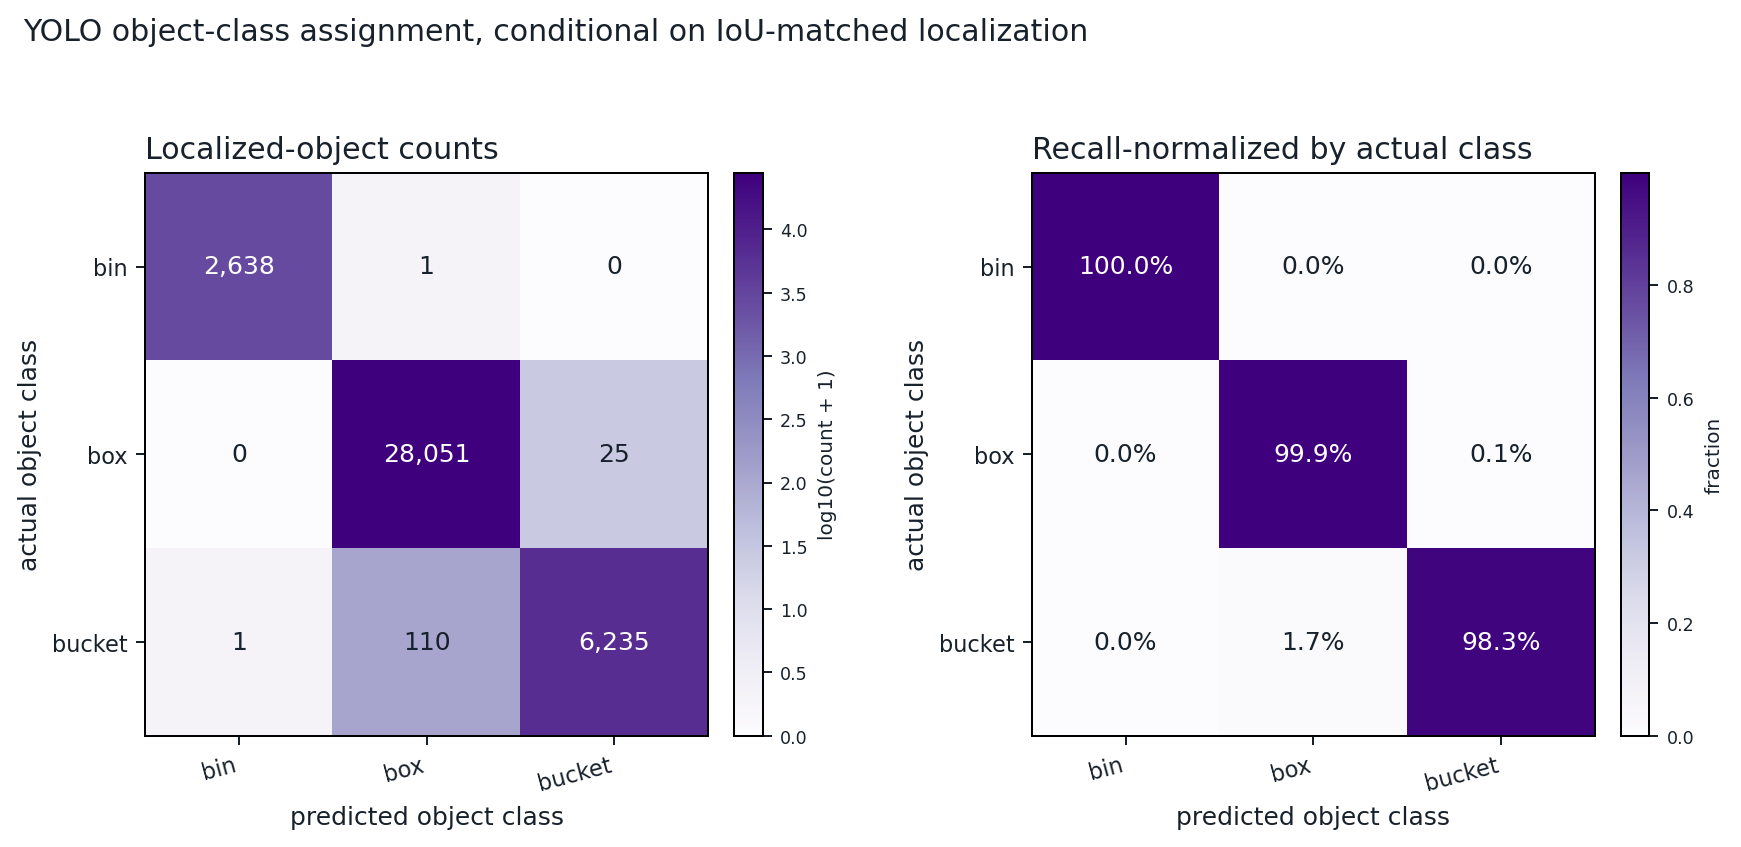
\includegraphics[width=\textwidth]{../../../output/yolo_eval/classification_confusion_light.png}
  \caption[Object-class confusion conditional on class-agnostic IoU association.]{Object-class confusion conditional on class-agnostic IoU association.
  Rows are actual object classes and columns are predicted object classes. The
  left panel gives counts on a logarithmic colour scale; the right panel
  normalizes within each actual class. Background is intentionally excluded.}
  \label{fig:yolo-classification-confusion}
\end{figure}
